Für das korrigierte $p_\text{T}$-Spektrum wird zuletzt noch die systematische Unsicherheit bestimmt.
Dabei wird sich in dieser Arbeit rein auf die systematische Unsicherheit, die durch Variation in der Peakextraktion kommt, fokussiert.
Das korrigierte $p_\text{T}$-Spektrum, das mit der Variation extrahiert wurde, wird mit dem korrigierten $p_\text{T}$-Spektrum ohne Variationen verglichen.
Die Variationen die in dieser Arbeit verwendet wurden lassen sich in vier Abschnitte unterteilen.
\newline
Bei der \textbf{Variation des Zählbereiches} und der \textbf{Variation des Parametrisierungsbereiches}, wird der Zähl- beziehungsweise Parametrisierungsbereich einmal ausgeweitet und ein anderes mal verkleinert.
Bei der Variation wird die untere Grenze jeweils um $0,01 \text{ GeV}/c^{2}$ verschoben, während die obere Grenze um $0,025 \text{ GeV}/c^{2}$ verändert wird, wie Tabelle \ref{tab:ParamAndIntRange} zeigt.
Die Änderung der unteren Grenze wurde so gewählt, dass das kombinierte Template des korrelierten Untergrunds die einzelnen Templates trotz der Anforderung an den Öffnungswinkel gut beschreibt.
Gleichzeitig wird sicher gestellt, dass der Teil des Signals, der aus Konversionselektronen oder Konversionspositronen besteht, möglichst vollständig im Zähl- beziehungsweise Parametrisierungsbereich liegt.
\begin{table}[b!]
\centering
\begin{tabular}{c|c||c||c|}
\cline{2-4}
                                                                      & Standard & Vergr{\"o}{\ss}ert & Verkleinert \\ \hline
\multicolumn{1}{|c|}{\multirow{2}{*}{$m_\text{inv}\text{ (GeV}/c)$}} & $0,06$   & $0,05$             & $0,07$      \\ \cline{2-4} 
\multicolumn{1}{|c|}{}                                                & $0,25$   & $0,275$            & $0,225$     \\ \hline
\end{tabular}
\caption{Obere und untere Grenze des Parametrisierungs- und Zählbereichs}
\label{tab:ParamAndIntRange}
\end{table}
\begin{figure}[t]
\centering
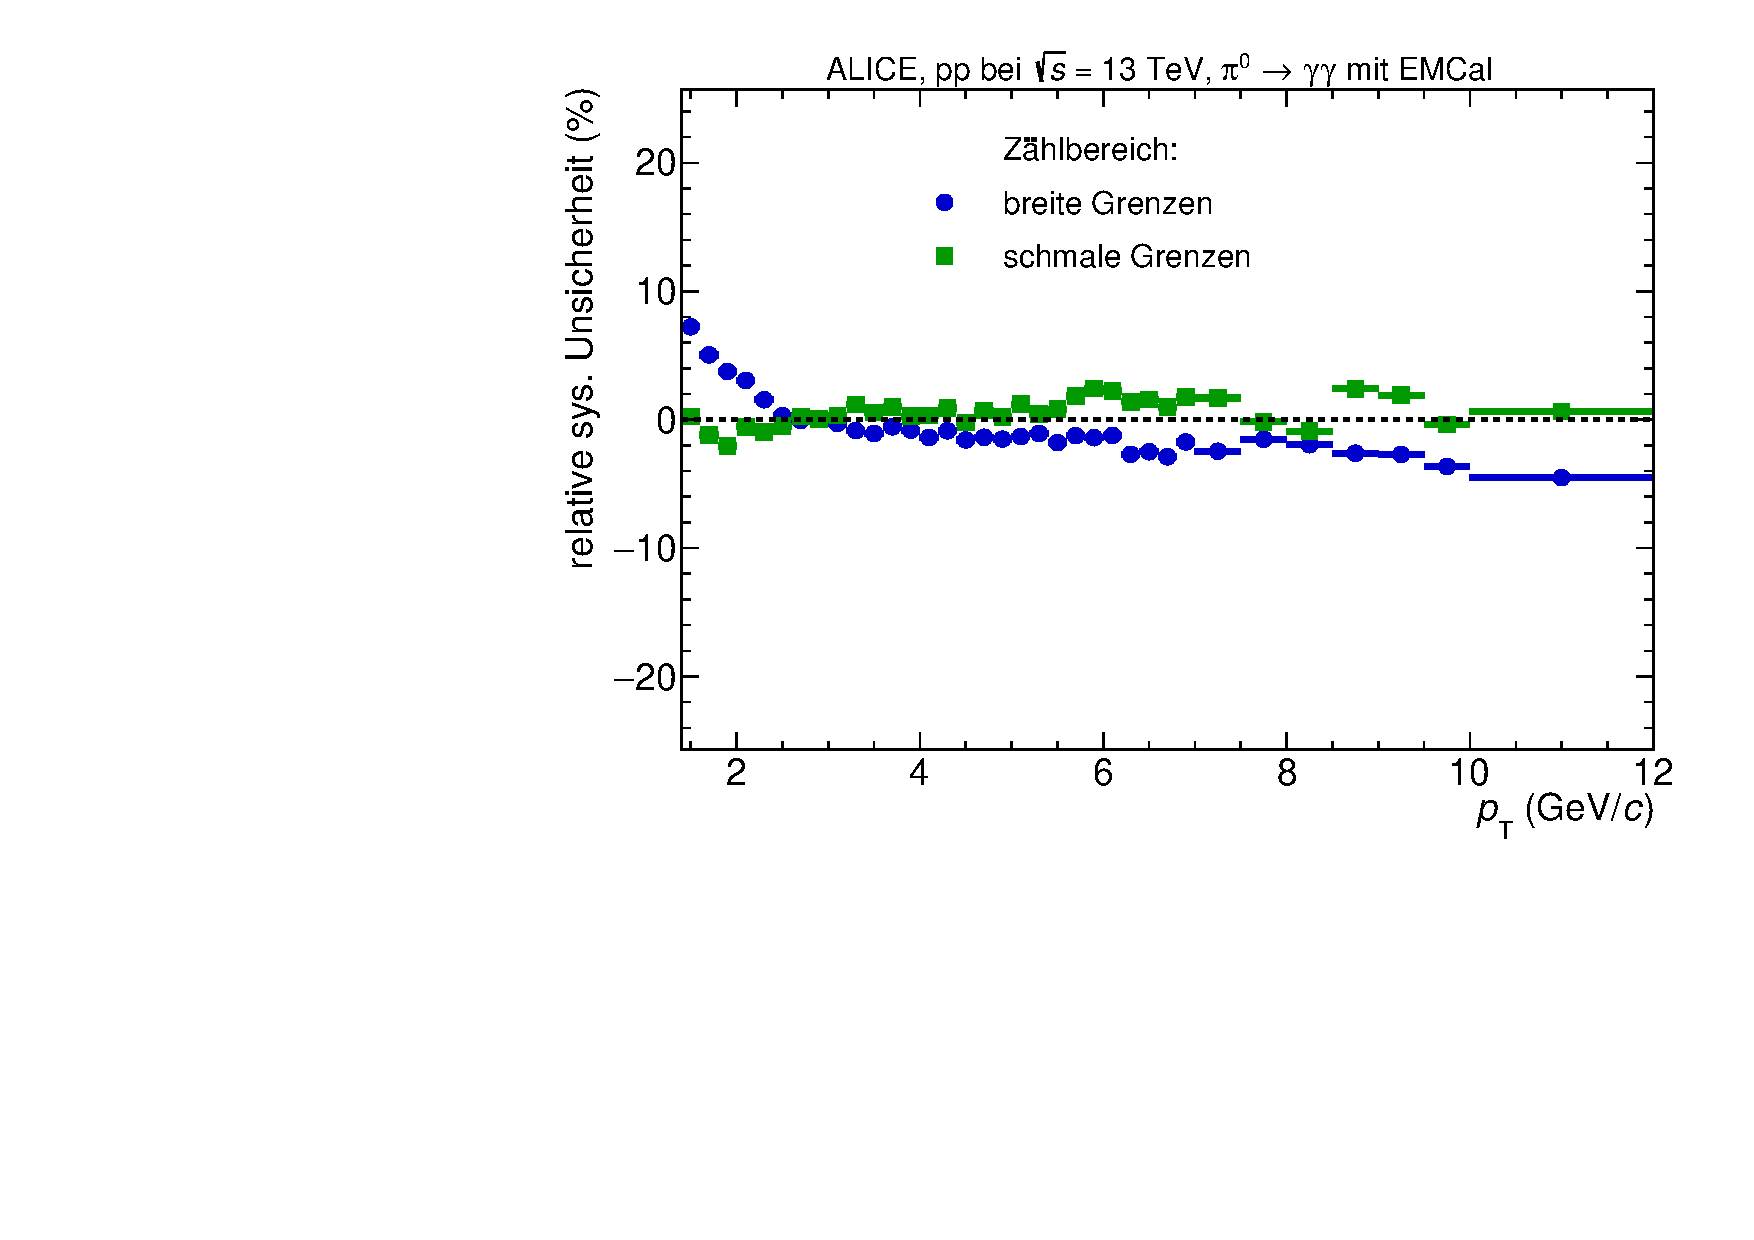
\includegraphics[width=.65\linewidth]{YieldsSysUncerIntRange_Data_2016.pdf}
\caption{Relative systematische Unsicherheit durch die Variation des Zählbereiches in Abhängigkeit von $p_\text{T}$.}
\label{fig:IntSys}
\end{figure}
\newline
Abbildung \ref{fig:IntSys} zeigt die relative systematische Abweichung für die Variation des Zählbereiches.
Beide Variationen weisen eine lineare Abweichung auf.
Die Abweichungen für breite Grenzen liegt ab $p_\text{T} > 5,8 \text{ GeV}/c$ im positiven Bereich, während die Abweichungen für schmale Grenzen dort im negativen liegen.
\begin{figure}[t!]
\centering
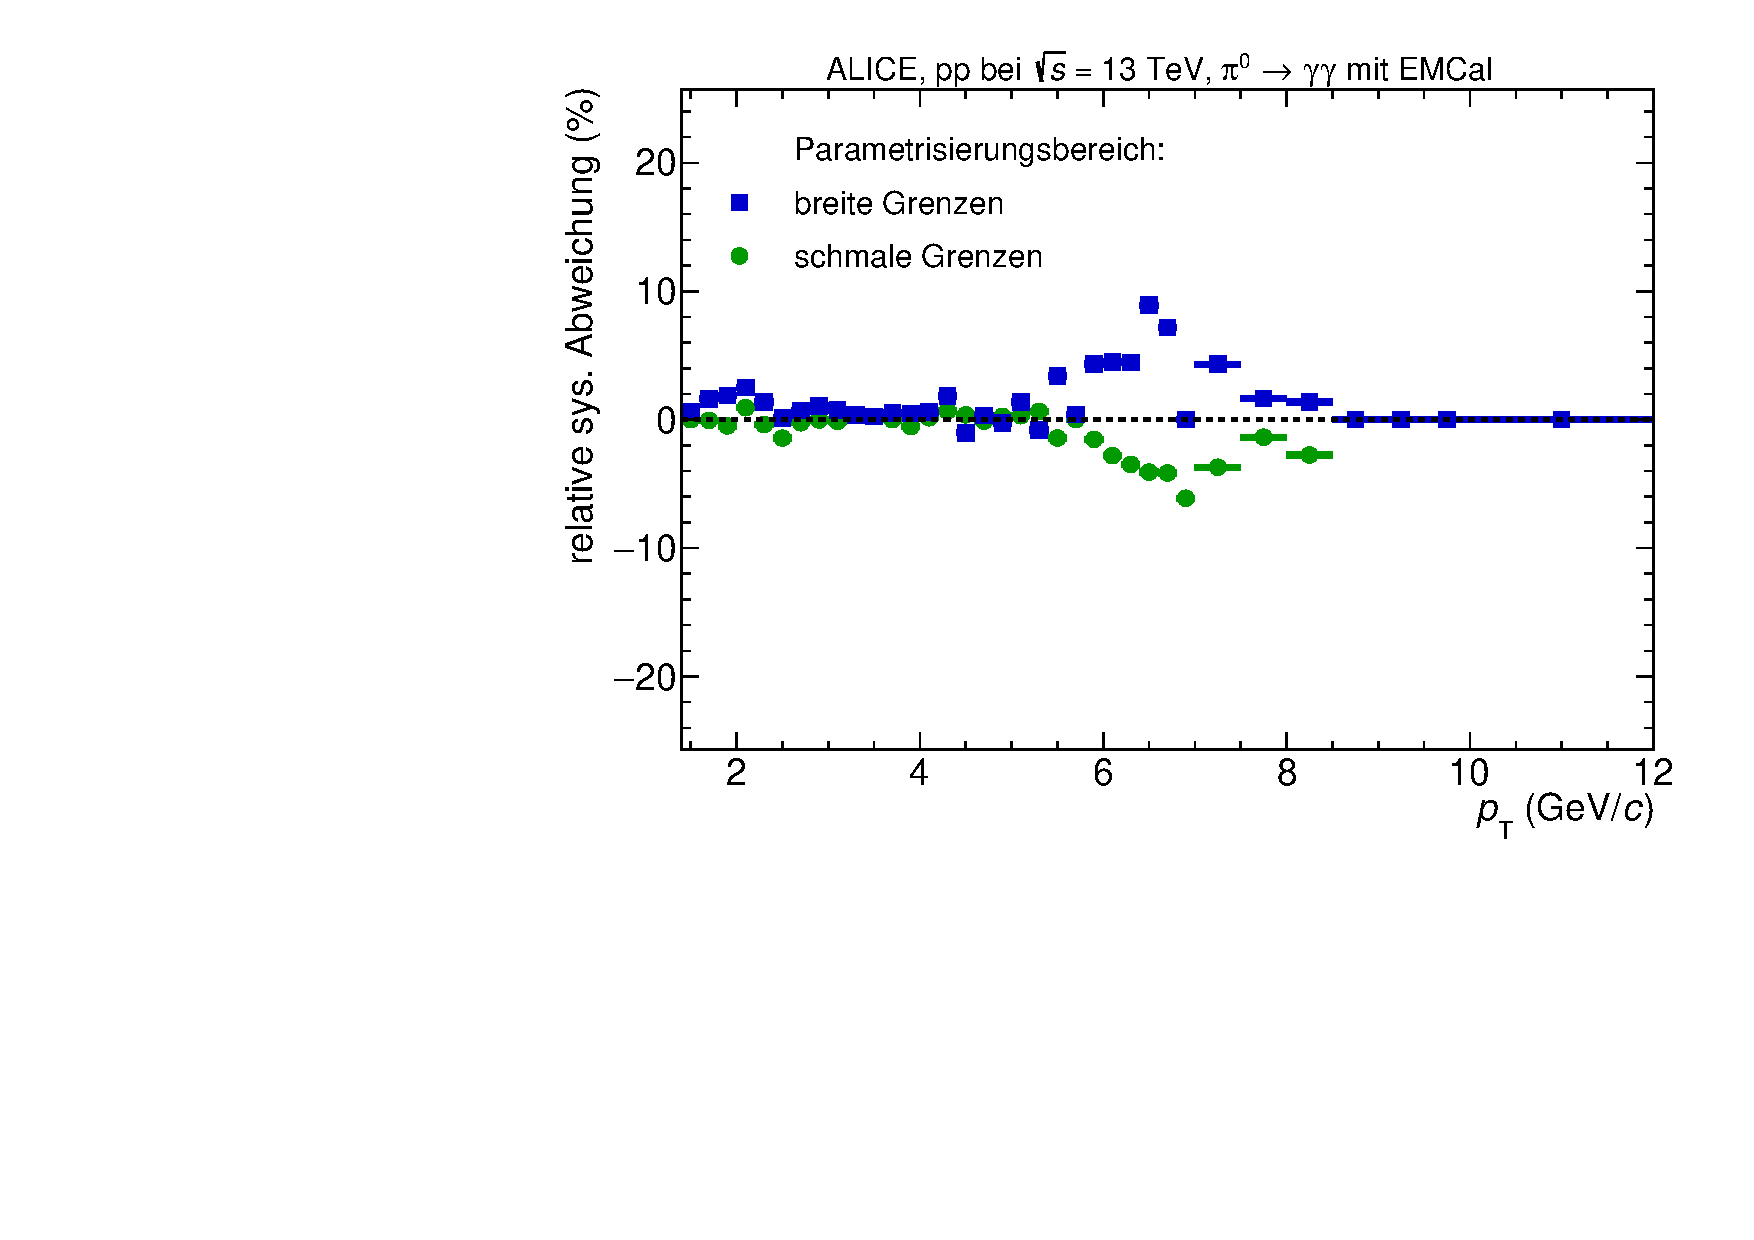
\includegraphics[width=.65\linewidth]{YieldsSysUncerFitRange_Data_2016.pdf}
\caption{Relative systematische Unsicherheit durch die Variation des Paramtrisierungsbereiches in Abhängigkeit von $p_\text{T}$.}
\label{fig:ParamSys}
\end{figure}
\newline
Abbildung \ref{fig:ParamSys} zeigt die relative systematische Unsicherheit für die Variation des Parametrisierungsbereiches.
Die Abweichungen befinden sich nahe der Null für schmale und breite Grenzen.
Eine Ausnahme bildet der $p_\text{T}$-Bereiches von $5,8 \text{ GeV}/c$ bis $7,5 \text{ GeV}/c$.
Dort liegen die Werte für breite Grenzen deutlich im positiven, die Werte für kleine Grenzen liegen hingegen im negativen Bereich.
\begin{figure}[t!]
\centering
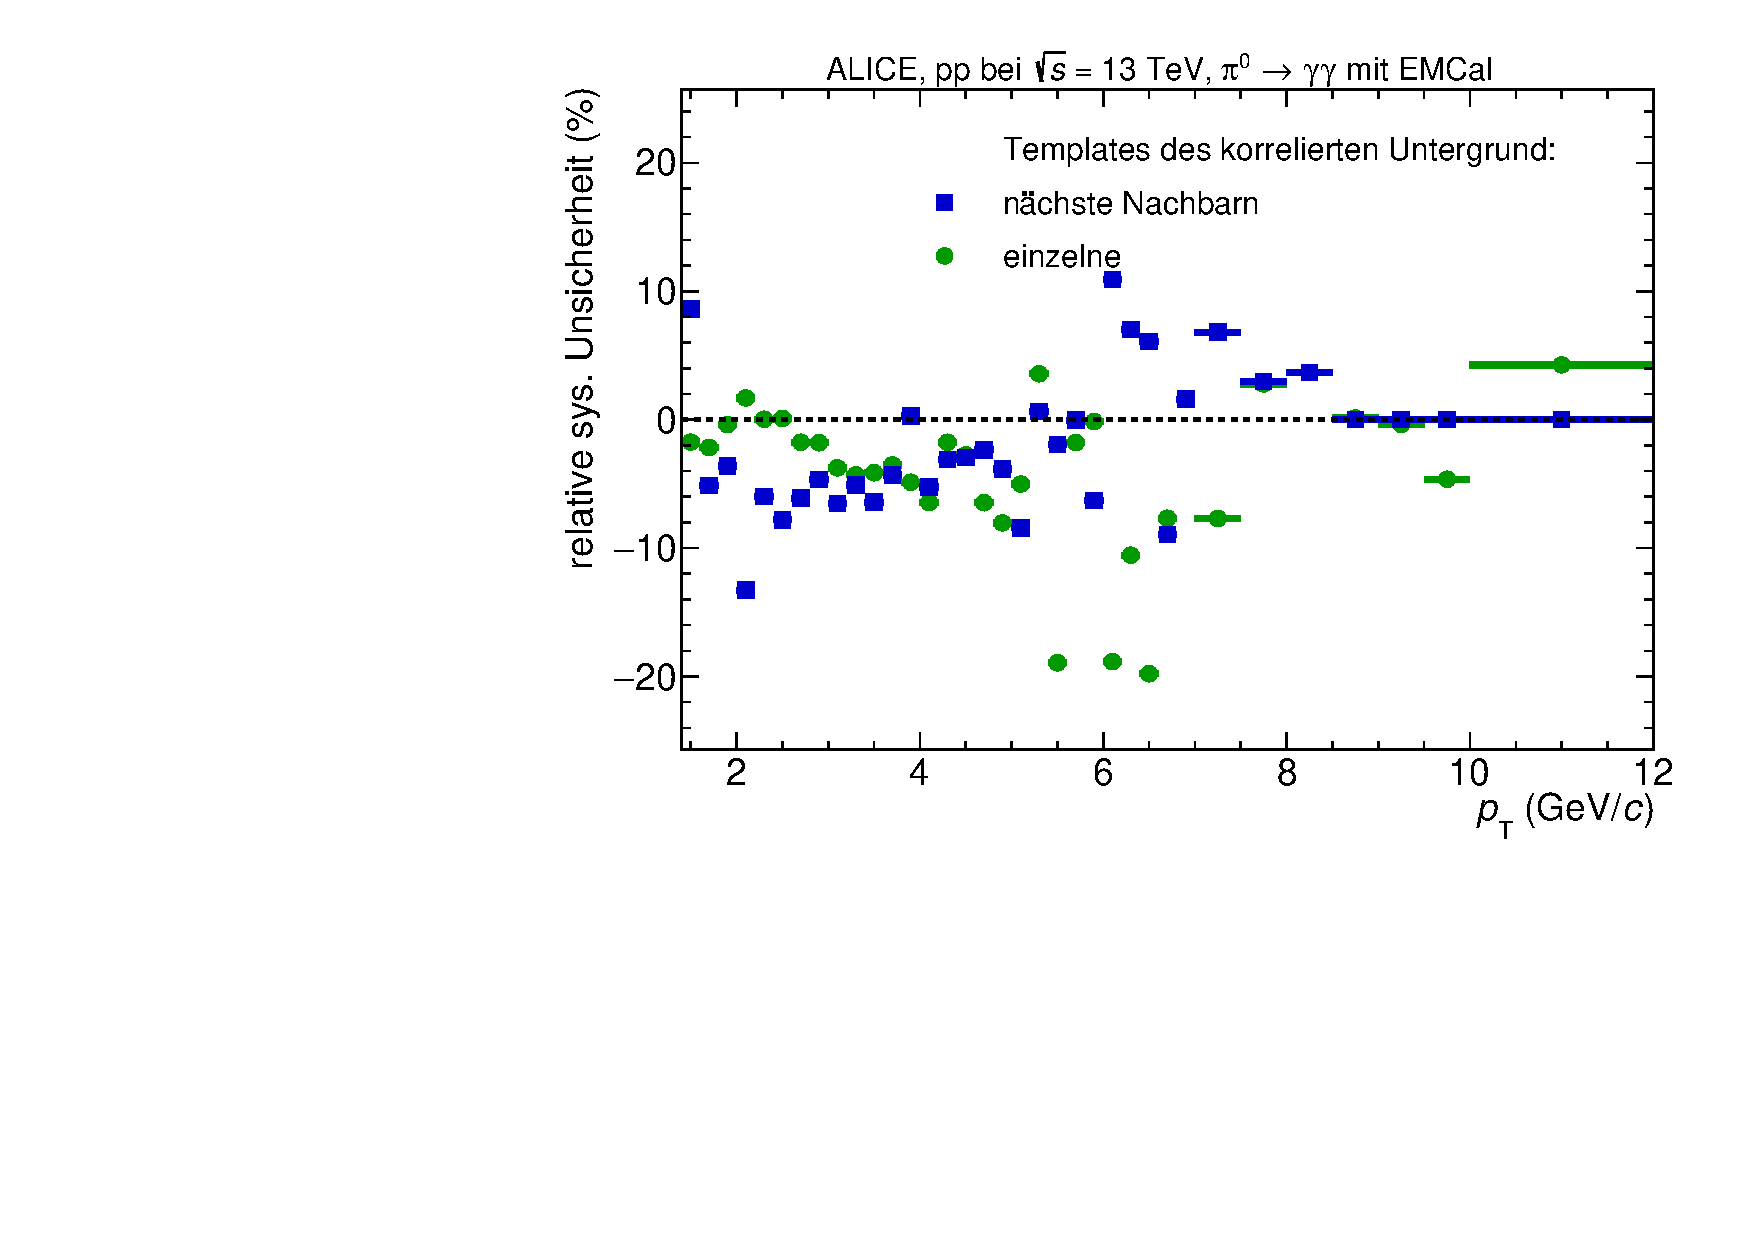
\includegraphics[width=.65\linewidth]{YieldsSysUncerBkgVariation_Data_2016.pdf}
\caption{Relative systematische Abweichung durch die Variation der Templates des korrelierten Untergrunds in Abhängigkeit von $p_\text{T}$.}
\label{fig:BkgSys}
\end{figure}
\newline
Die \textbf{Variation der Templates des korrelierten Untergrunds} basiert auf den in Abschnitt \ref{s3s5s2} vorgestellten Methoden zur Bestimmung der Templates des korrelierten Untergrunds.
Für kleine $p_\text{T}$ von $1,4 \text{ GeV}/c$ bis $4,4 \text{ GeV}/c$ zeigen beide Methoden eine geringe Abweichung.
Der $p_\text{T}$-Bereich von $4,4 \text{ GeV}/c$ bis $7,5 \text{ GeV}/c$ hingegen weist starke Abweichungen für beide Methoden auf.
Die Methode mit einzelnen Templates des korrelierten Untergrunds unterschätzt in diesem Bereich die Anzahl produzierter $\pi^{0}$ im Vergleich zur Methode mit kombiniertem Template des korrelierten Untergrunds stark.
Die Ursache hierfür liegt vor allem in der großen statischen Unsicherheit der einzelnen Templates des korrelierten Untergrunds.
Durch diese Unsicherheit wird der korrelierte Untergrund überschätzt.
Bei der Methode mit den nächsten Nachbarn wird der korrelierten Untergrund hingegen unterschätzt, weshalb dort die Abweichung im positiven Bereich liegt.
\begin{figure}[t!]
\centering
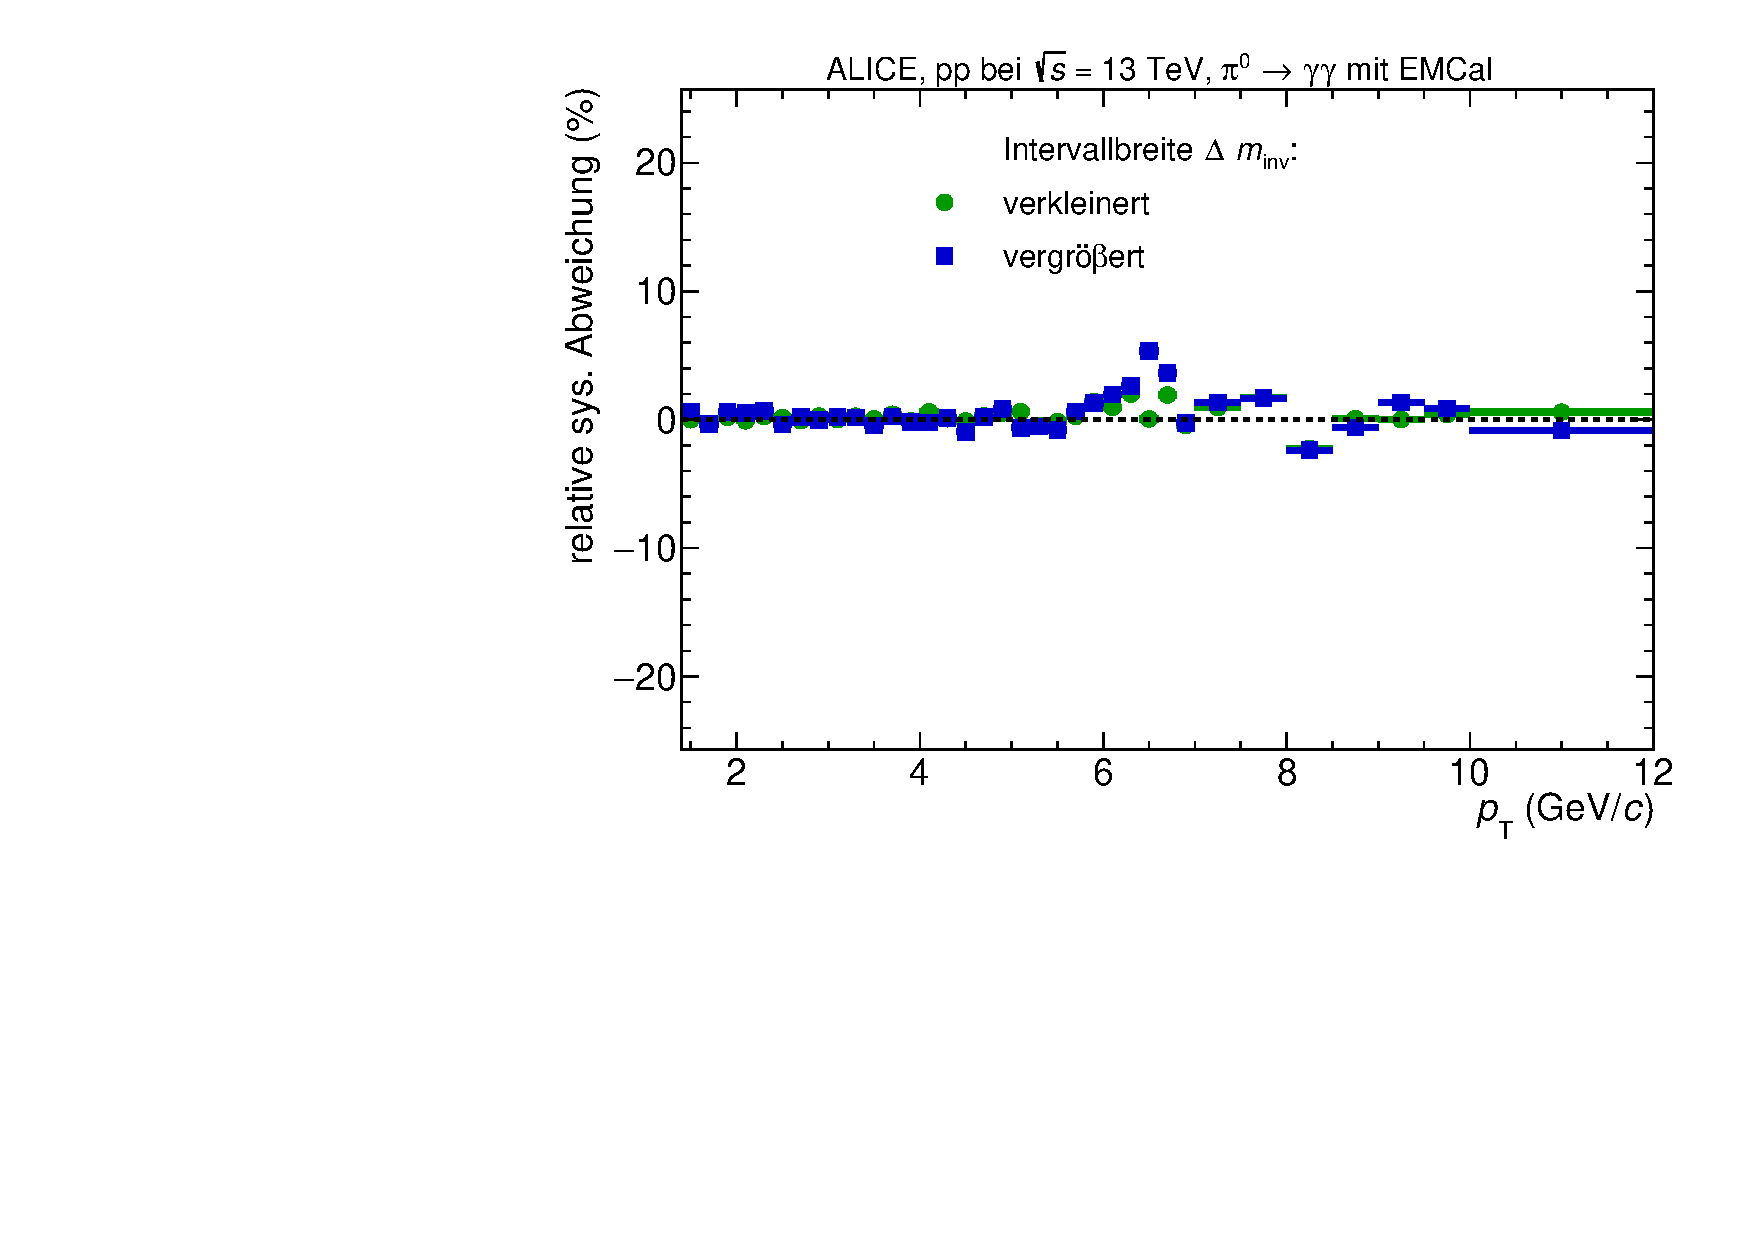
\includegraphics[width=.65\linewidth]{YieldsSysUncerRebinning_Data_2016.pdf}
\caption{Relative systematische Abweichung durch die Variation von $\Delta m_\text{inv}$ in Abhängigkeit von $p_\text{T}$.}
\label{fig:BinningSys}
\end{figure}
\newline
Die Breite der $m_\text{inv}$-Intervalle $\Delta m_\text{inv}$ wird in der \textbf{Variation von} $\boldsymbol{\Delta m}_\textbf{inv}$ verändert.
Tabelle \ref{tab:Binning} zeigt $\Delta m_\text{inv}$ wie es für diese Analyse gewählt wurde, sowie für die Variationen.
Dabei hängt $\Delta m_\text{inv}$ zusätzlich von $p_\text{T}$ ab.
\newline
Beide Variationen zeigen kaum Abweichungen, lediglich im $p_\text{T}$-Bereich von $6,0 \text{ GeV}/c$ bis $7,5 \text{ GeV}/c$ bildet sich eine deutliche Abweichung für vergrößerte $\Delta m_\text{inv}$ ab.
\begin{table}[b!]
\centering
\begin{tabular}{c|c|c|}
\cline{2-3}
                                                          & $\Delta m_\text{inv}$ $\left(\text{GeV}/c^{2}\right)$ & $p_\text{T}$-Intervall $\left(\text{GeV}/c\right)$ \\ \hline
\multicolumn{1}{|c|}{\multirow{3}{*}{Standard}}           & $0\,004$                                              & $1\,4-7\,5$                                        \\ \cline{2-3} 
\multicolumn{1}{|c|}{}                                    & $0\,008$                                              & $7\,5-10$                                          \\ \cline{2-3} 
\multicolumn{1}{|c|}{}                                    & $0\,010$                                              & $10-12$                                            \\ \hline \hline
\multicolumn{1}{|c|}{\multirow{3}{*}{Vergr{\"o}{\ss}ert}} & $0\,005$                                              & $1\,4-7\,5$                                        \\ \cline{2-3} 
\multicolumn{1}{|c|}{}                                    & $0\,010$                                              & $7\,5-10$                                          \\ \cline{2-3} 
\multicolumn{1}{|c|}{}                                    & $0\,020$                                              & $10-12$                                            \\ \hline \hline
\multicolumn{1}{|c|}{\multirow{3}{*}{Verkleinert}}        & $0\,002$                                              & $1\,4-7\,5$                                        \\ \cline{2-3} 
\multicolumn{1}{|c|}{}                                    & $0\,005$                                               & $7\,5-10$                                          \\ \cline{2-3} 
\multicolumn{1}{|c|}{}                                    & $0\,008$                                              & $10-12$                                            \\ \hline
\end{tabular}
\caption{Die verschiedenen Breiten der $m_\text{inv}$-Intervalle $\Delta m_\text{inv}$ in Abhängigkeit von $p_\text{T}$.}
\label{tab:Binning}
\end{table}
\begin{figure}[t!]
\centering
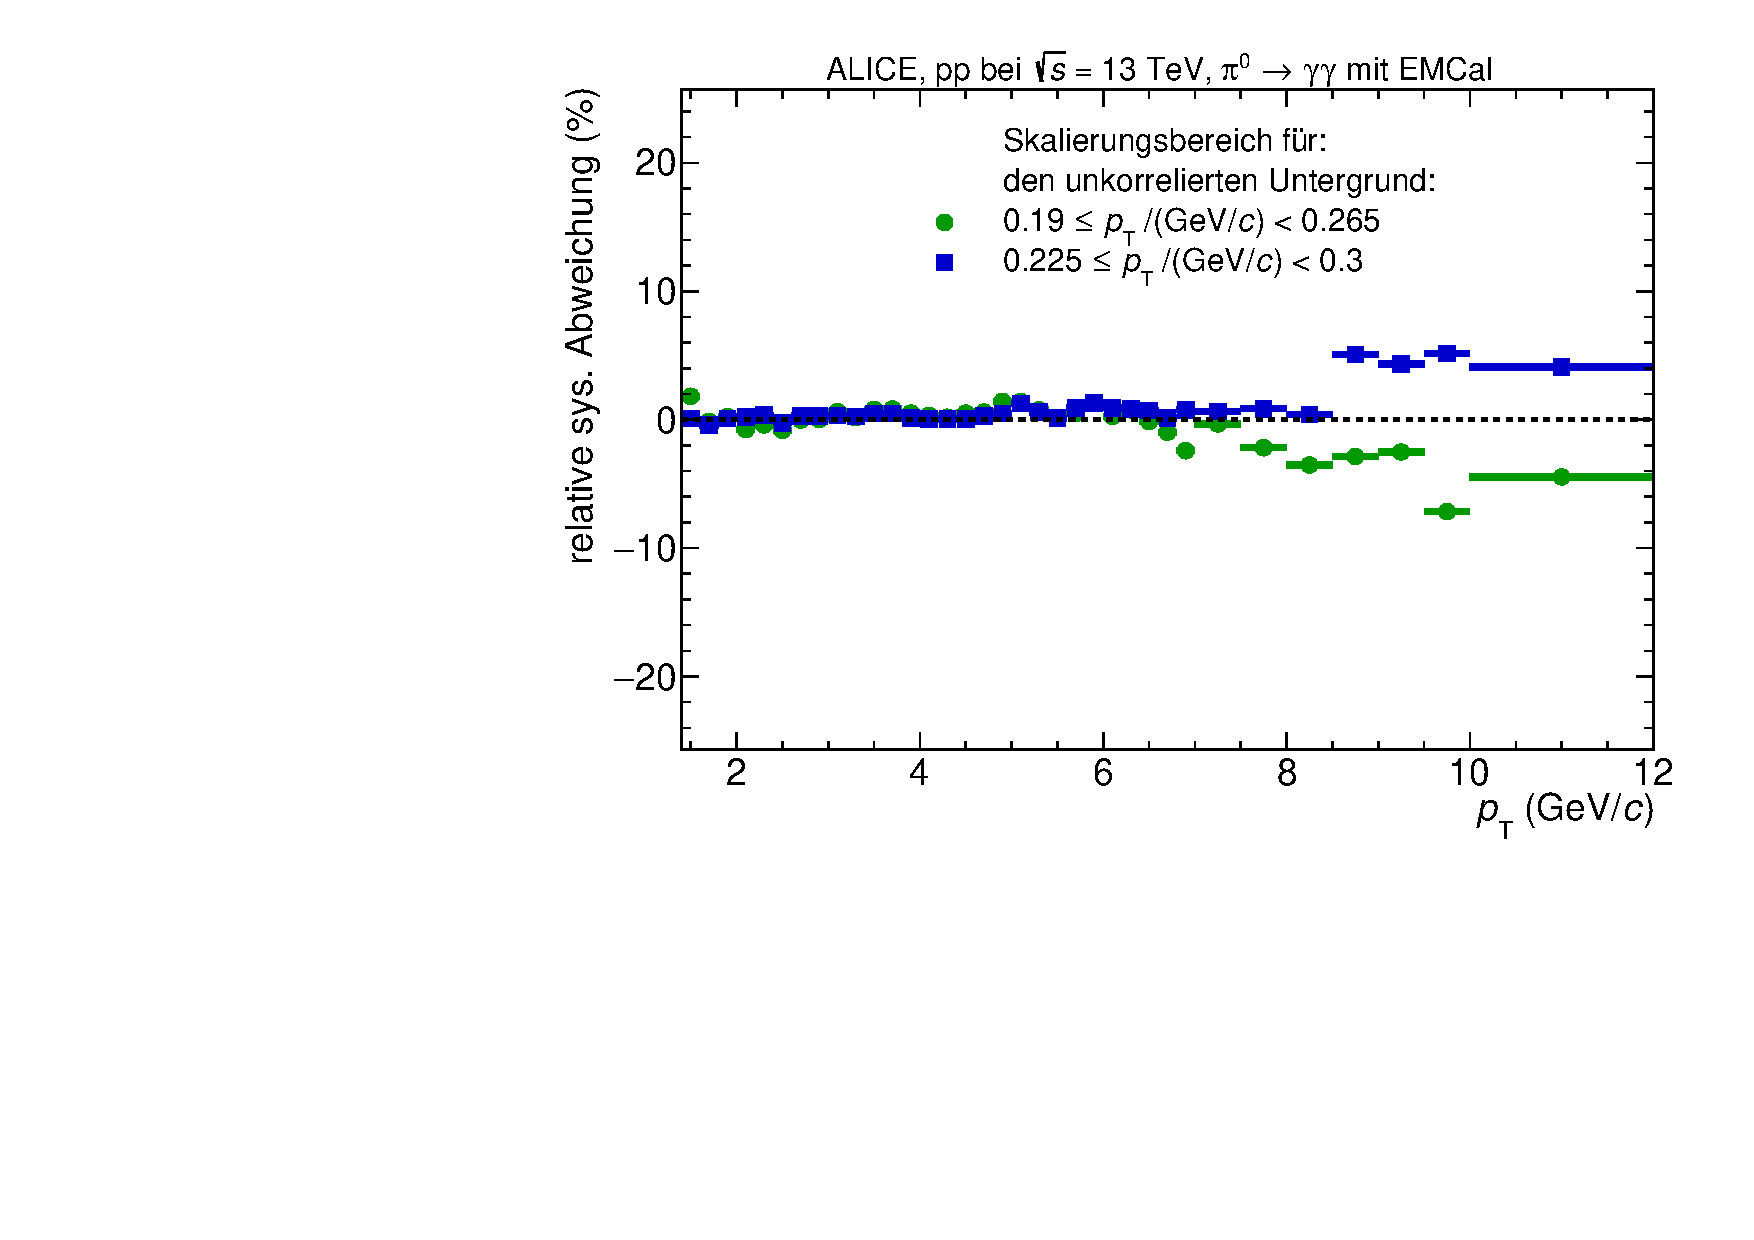
\includegraphics[width=.65\linewidth]{YieldsSysUncerUncorrBkgVariation_Data_2016.pdf}
\caption{Relative systematische Abweichung durch die Variation des Parametrisierungsbereiches des unkorrelierten Untergrunds in Abhängigkeit von $p_\text{T}$.}
\label{fig:LeftBkgSys}
\end{figure}
\newline
Bei der \textbf{Variation des Parametrisierungsbereiches des unkorrelierten Untergrunds} wird der Bereich verändert, indem die \textit{mixed Event} Verteilung skaliert wird.
Abbildung \ref{fig:LeftBkgSys} zeigt die zugehörigen Abweichungen.
Bis $p_\text{T} = 7,5 \text{ GeV}/c$ weisen beide Abweichungen einen linearen Verlauf um Null rum auf.
Ab $p_\text{T} = 7,5 \text{ GeV}/c$ weicht die Variation, bei der die obere Grenze nach unten verschoben wurde, ins negative ab.
Die Variation, bei der die untere Grenze verändert wurde, zeigt eine positive Abweichung, wobei diese erst ab $p_\text{T} = 8,5 \text{ GeV}/c$ auftritt.
\begin{figure}[t!]
\centering
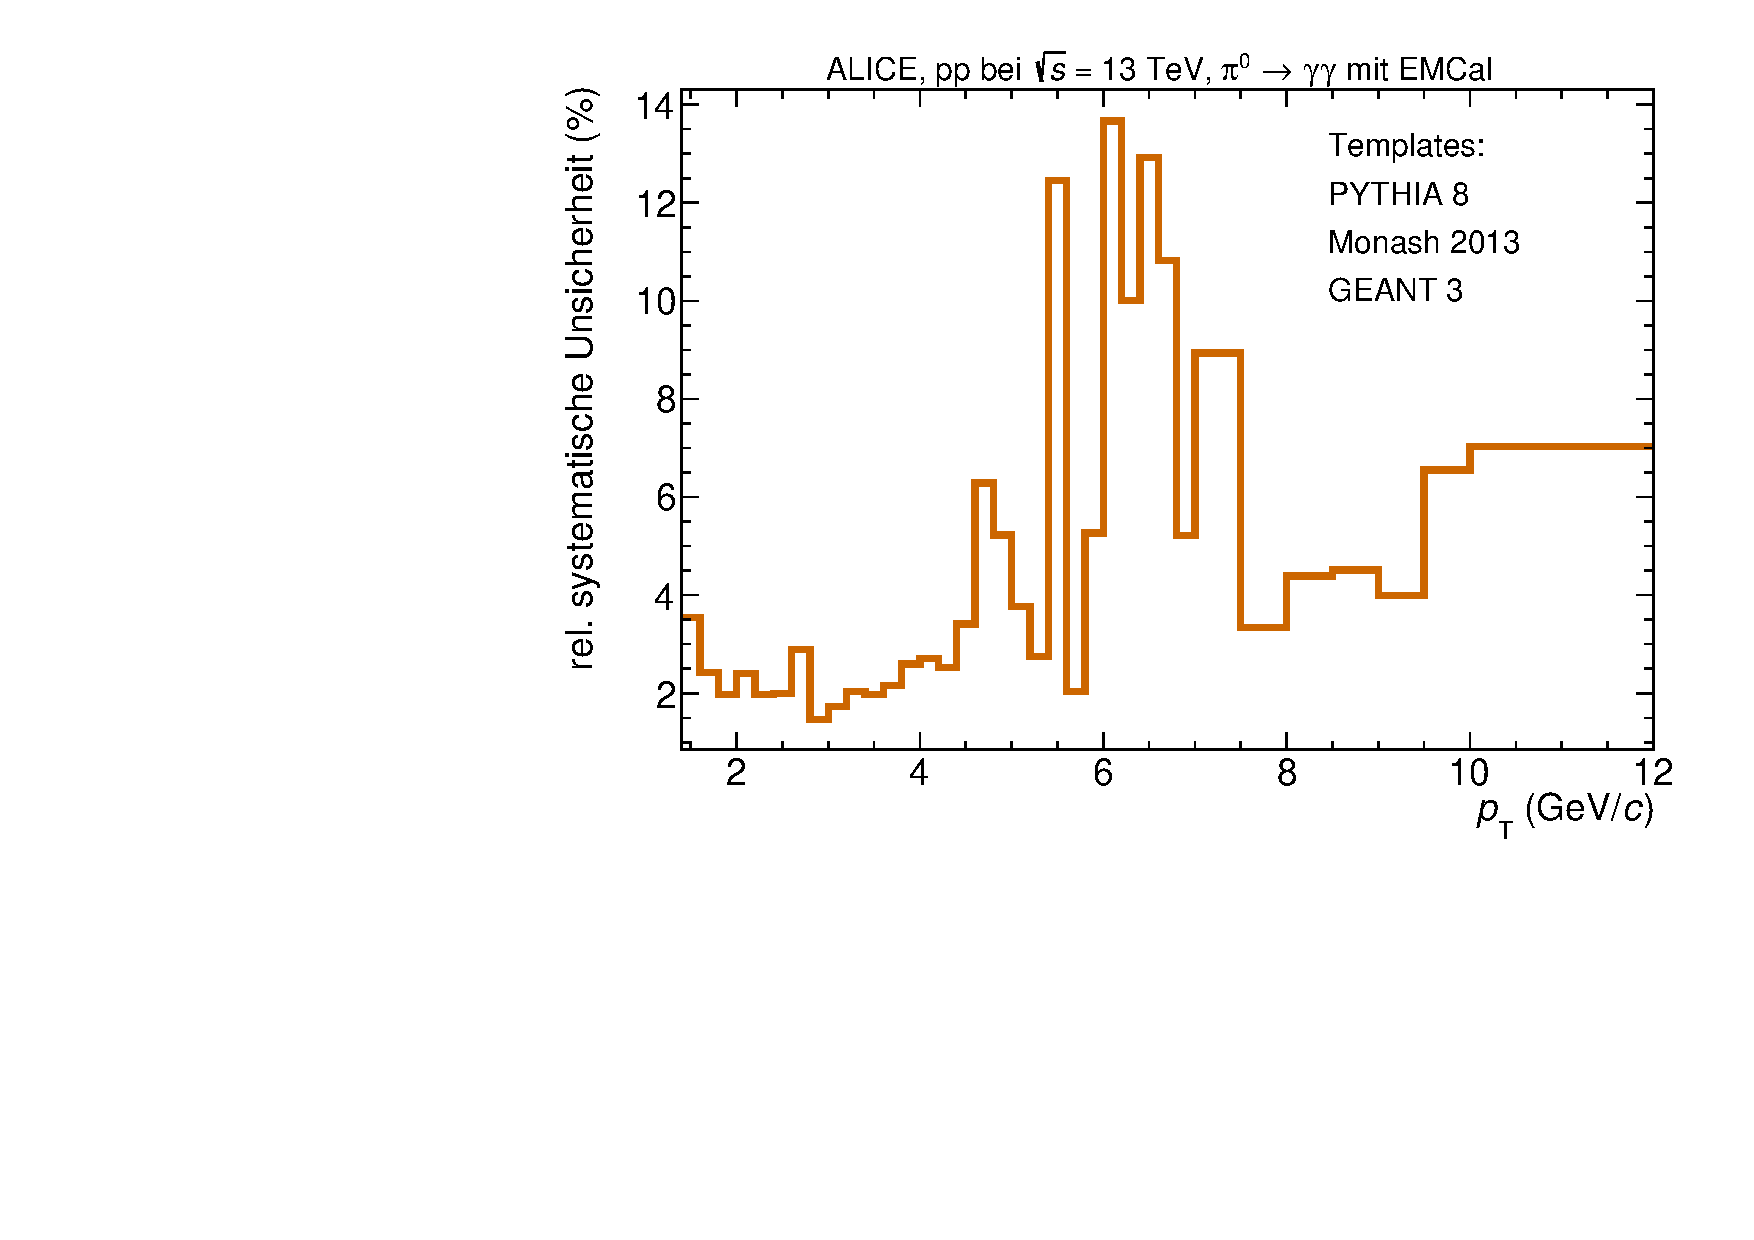
\includegraphics[width=.65\linewidth]{SystematischeUnsicherheit_Data_2016.pdf}
\caption{Gesamte relative systematische Unsicherheit des korrigierten $\pi^ {0}$-Spektrums.}
\label{fig:SysUncer}
\end{figure}
\newline
Zur Bestimmung der systematischen Unsicherheit $\sigma_{i,j}$ einer Variationsart $j$ in einem $p_\text{T}$-Intervall $i$ wird das quadratische Mittel der relativen Abweichungen der $n$ unterschiedlichen Variationen $k$ verwendet.
Es gilt:
\begin{align}
\sigma_{i,j} = \sqrt{\frac{1}{n}\sum_{k=1}^{n}\left(\Delta y_{i,j,k}\right)^{2}}
\end{align}
Die gesamte Systematische Unsicherheit $\sigma_{i}$ in einem $p_\text{T}$-Intervall $i$ ergibt sich durch quadratische Addition der systematischen Unsicherheiten der fünf Variationsarten $\sigma_{i,j}$.
\begin{align}
\sigma_{i} = \sqrt{\sum_{j=1}^{n}\left(\sigma_{i,j}\right)^{2}}
\end{align}
Abbildung \ref{fig:SysUncer} zeigt die gesamte relative systematische Unsicherheit in Abhängigkeit von $p_\text{T}$.
Für kleine $p_\text{T}$ im Bereich von $1,4 \text{ GeV}/c$ bis $4,5 \text{ GeV}/c$ liegt die systematischen Unsicherheit zwischen dem Minimalwert von etwa $0,8\%$ und $1,6\%$.
Danach steigt die systematische Unsicherheit mit größerem $p_\text{T}$ an.
Besonders der $p_\text{T}$-Bereich von $4,4 \text{ GeV}/c$ bis $7,5 \text{ GeV}/c$ zeigt hierbei starke Schwankungen auf, die hauptsächlich durch die Variation der Templates des korrelierten Untergrunds, sowie der Änderung des Parametrisierungsbereiches kommen.
In diesem Bereich liegt auch das Maximum mit einer systematischen Unsicherheit von etwa $6\%$.
Die systematische Unsicherheit ab $p_\text{T} = 7,5 \text{ GeV}/c$ wird von der Variation des Parametrisierungsbereiches des unkorrelierten Untergrunds dominiert.
\begin{figure}[t!]
\centering
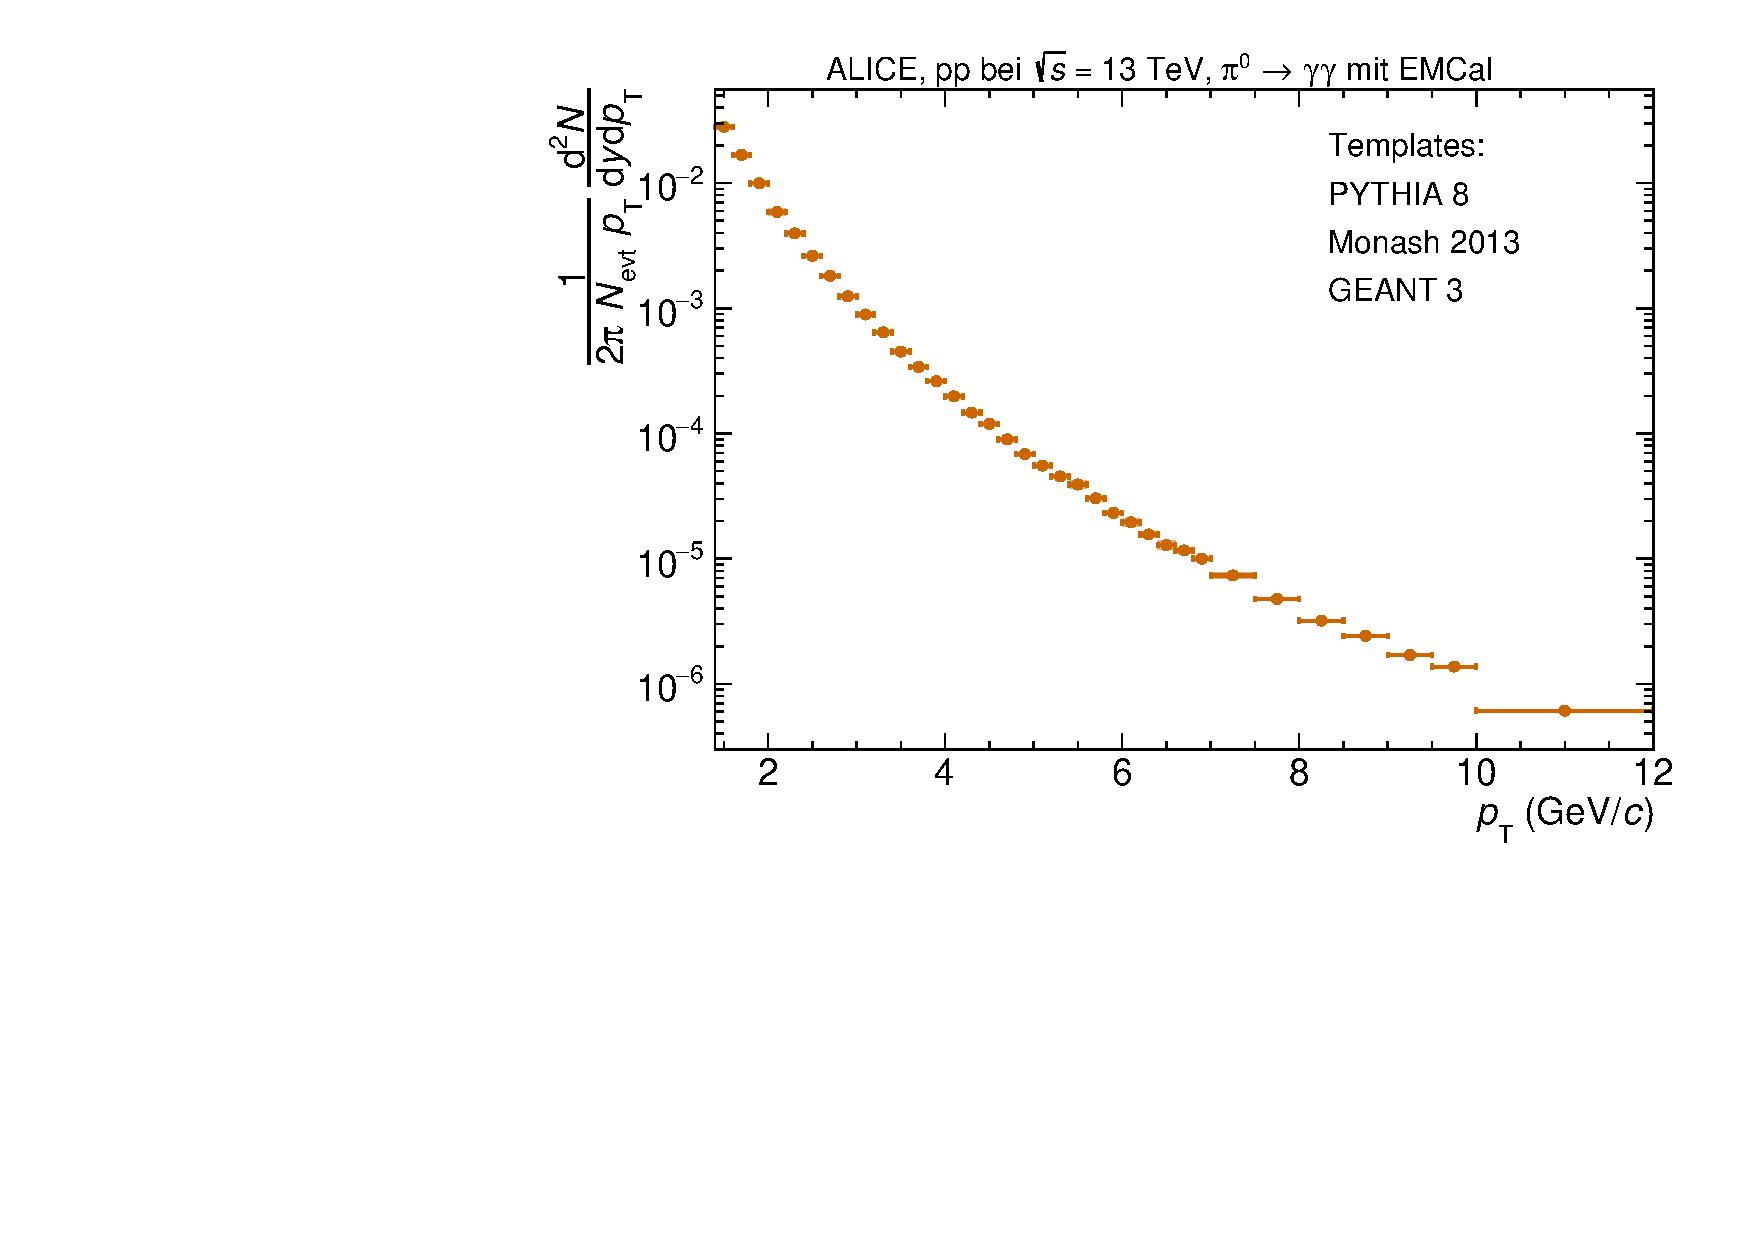
\includegraphics[width=.65\linewidth]{KorrigierterYield_Data_2016.pdf}
\caption{Korrigiertes $p_\text{T}$-Spektrum mit systematischer und statistischer Unsicherheit.}
\label{fig:KorrYield}
\end{figure}
\newline
Abbildung \ref{fig:KorrYield} zeigt das korrigierte $p_\text{T}$-Spektrum mit statistischer und systematischer Unsicherheit.
Die statistische Unsicherheit wird durch die vertikalen Linien, die systematische Unsicherheit durch die farbigen Boxen dargestellt.
\newline
Das korrigierte $p_\text{T}$-Spektrum wird im folgenden Abschnitt mit dem Ergebnis der Standardmethode verglichen.